\section{The Architect's Question}\label{the-architects-question}

After this chapter we should be able to answer the architect's
fundamental constraint question: \emph{does the model and its context
fit in the memory floor before we ask whether it can compute or
communicate?} We will build the arithmetic for the KV cache from first
principles, reconcile it with the canonical \textasciitilde1.3 MB/token
figure from \hyperref[chap:1]{Chapter 1}, and contrast inference residency (weights + KV)
with fine-tuning residency (weights + gradients + optimizer states). The
goal is to make ``does it fit?'' a concrete, quantified check --- not a
back-of-the-envelope guess. Throughout, the arithmetic anchors to the
canonical enterprise-Q\&A RAG scenario (§14): \textasciitilde10 rps
average / \textasciitilde40 rps peak traffic (2,000 registered users ×
5\% concurrency → 100 concurrent → \textasciitilde10 rps via Little's
Law; peaks at 20\% concurrency → \textasciitilde40 rps) served by a 70B
FP16 model on an 8×H100 host. KV-cache per-token figures are given at
the referenced precision throughout: \textasciitilde1.3 MB/token at
\textbf{8-bit}, \textasciitilde2.5 MB/token at \textbf{FP16}; the
canonical scenario's headline \textasciitilde1.3 MB/token figure is the
8-bit variant.

\section{Concept}\label{concept}

Memory is the first constraint because every LLM workload begins with a
residency check: can the model and its active data structures be placed
on the target hardware? The KV cache is the primary expression of this
constraint during inference: it grows linearly with context length, and
its size depends on the model's layer count, hidden dimension, and the
precision chosen for key and value storage. Unlike FLOPs, which scale
with operations per token, the KV cache occupies memory continuously for
the lifetime of a request --- it is always resident, always consuming
HBM bandwidth for every re-read. The architect must therefore size two
distinct memory loads: the static weight footprint and the dynamic KV
footprint that varies with prompt length. Quantization (FP8, FP4, 2-bit
asymmetric) reduces both, but the KV cache is the one component that
does not shrink as aggressively as weights --- per-block scale/offset
metadata and per-token variation mean the memory reduction is typically
40--50\% rather than the 2×--4× seen in weight-only quantization. The
residency floor is therefore set by weights + KV (+ activations, in
fine-tuning), and the architect's first question is whether this sum
fits on the target GPUs. This is why ``does it fit?'' is the architect's
primary gate: before we ask whether the model can compute or
communicate, we must first establish that the working set --- weights
plus the context-dependent KV state --- resides on-GPU. If it does not,
every subsequent decision (offload, recompute, page) is a degradation,
not a cost-optimization.

The residency floor has two distinct regimes. Inference, the floor is
weights + KV: the model's static parameters plus the context-dependent
key/value tensors that grow with every token added to the prompt. In
fine-tuning, the floor rises further to weights + gradients + optimizer
states, because every parameter update requires its own momentum and
velocity vectors (Adam) or per-parameter scaling (LAMB/RMSProp). The
contrast between these two floors --- inference typically 160--200 GB
for a 70B model at FP16 with 9.2K context {[}2° DERIVED{]}, fine-tuning
exceeding 1 TB {[}2° DERIVED{]} --- is the architect's central
memory-takeaway.

\section{Mental Model}\label{mental-model}

Think of the KV cache as \textbf{per-request state that survives for the
duration of a single forward pass} --- unlike weights, which are loaded
once and reused across requests, the KV cache is allocated per request
and grows with every token added to the context. A 9.2K prompt on a 70B
model at FP16 carries \textasciitilde24 GB of KV state that must be
on-GPU for the entire prefill + decode sequence. If it does not fit, the
serving stack must page, offload, or recompute --- each option degrades
latency or throughput. The durable mental model is: \emph{every token we
add to the context exacts a fixed memory toll, and that toll is paid in
HBM every time the GPU re-reads the cache during decode.} This is why
context length is the single most powerful lever on inference memory
pressure, and why ``does it fit?'' is the architect's primary gate.

\section{Worked Example}\label{worked-example}

We anchor all arithmetic in the canonical scenario (§14 of
book-architecture.md): a 70B-class dense model, FP16 weights (2 bytes
per parameter), 8 × GPUs (80 GB each, 640 GB total VRAM),
\textasciitilde9.2K input tokens + 300 output tokens. We compute
KV-cache size per token, total KV for the canonical context, and
contrast with long-context variants.

\textbf{\hyperref[tab:7.1]{Table 7-1}} --- KV-cache size per token and per-context
arithmetic for a 70B-class dense model at FP16. \emph{(All per-context
KV totals, residency figures, and fit/non-fit verdicts below are {[}2°
DERIVED{]} from the per-token formula 2 × layers × hidden\_dim × bytes;
model-card architecture constants are {[}1P: model card{]}.)}

\begin{longtable}[]{@{}
  >{\raggedright\arraybackslash}p{0.3333\linewidth}
  >{\raggedright\arraybackslash}p{0.3333\linewidth}
  >{\raggedright\arraybackslash}p{0.3333\linewidth}@{}}
\toprule\noalign{}
\begin{minipage}[b]{\linewidth}\raggedright
metric
\end{minipage} & \begin{minipage}[b]{\linewidth}\raggedright
value
\end{minipage} & \begin{minipage}[b]{\linewidth}\raggedright
derivation
\end{minipage} \\
\midrule\noalign{}
\endhead
\bottomrule\noalign{}
\endlastfoot
layers & 80 & canonical 70B full-MHA teaching model {[}1P:
canonical-workload.yaml{]} \\
hidden\_dim & 8192 & canonical 70B full-MHA teaching model {[}1P:
canonical-workload.yaml{]} \\
bytes per parameter (FP16) & 2 & FP16 = 2 bytes/param {[}1P:
facts/quantization.md Q3{]} \\
KV cache per token per layer & 2 × hidden\_dim × bytes & one key + one
value per layer \\
KV cache per token (FP16) & 2 × 80 × 8192 × 2 B ≈ 2.5 MB & = 2,560 KB;
rounded \\
KV cache per token (8-bit) & 2 × 80 × 8192 × 1 B ≈ 1.3 MB & = 1,280 KB;
reconciles with Ch.1 \\
9.2K input KV cache & 9,200 × 2.5 MB ≈ 23.9 GB & 9,200 × 2,560 KB \\
300 output KV cache & 300 × 2.5 MB ≈ 0.75 GB & 300 × 2,560 KB \\
total inference KV (9.2K + 300) & ≈ 24.7 GB & weights 140 GB + KV 24.7
GB ≈ 164.7 GB \\
32K input KV cache & 32,000 × 2.5 MB ≈ 80.0 GB & long-context variant \\
128K input KV cache & 128,000 × 2.5 MB ≈ 320.0 GB & aggressive
long-context variant \\
70B FP16 weights & 70B × 2 B = 140 GB & {[}1P: DERIVED from 70B × 2
bytes{]} \\
inference residency (weights + KV, 9.2K input) & ≈ 164.7 GB & 140 + 24.7
GB \\
inference residency (weights + KV, 32K input) & ≈ 220.0 GB & 140 + 80.0
GB \\
inference residency (weights + KV, 128K input) & ≈ 460.0 GB & 140 +
320.0 GB \\
2×H100 total VRAM & 2 × 80 GB = 160 GB & {[}1P: facts/serving.md
S8{]} \\
8×H100 total VRAM & 8 × 80 GB = 640 GB & {[}1P: facts/serving.md
S8{]} \\
fits 2×H100 at 9.2K? & no, 164.7 GB \textgreater{} 160 GB & requires
≥2×H100 with small overflow \\
fits 8×H100 at 9.2K? & yes & 164.7 GB \textless{} 640 GB \\
fits 8×H100 at 32K? & yes & 220.0 GB \textless{} 640 GB \\
fits 8×H100 at 128K? & yes, barely & 460.0 GB \textless{} 640 GB \\
fits 1×H100 at 9.2K? & no & 164.7 GB \textgreater{} 80 GB; needs
≥2×H100 \\

\label{tab:7.1}\end{longtable}

\emph{Note on ``does it fit?'': this residency check answers a
single-request question --- does ONE request's weights + KV fit in the
pool? It says nothing yet about how many such requests fit concurrently.
For that, an architect must subtract the runtime/activation/workspace
floor (\textasciitilde64 GB on the 8×H100 host) from the 640 GB pool
before sizing KV. We compute that concurrent capacity --- the
\textasciitilde436 GB KV budget and \textasciitilde18 requests/host ---
in \hyperref[chap:17]{Chapter 17}. Keep the two numbers separate: the \textasciitilde500 GB
headroom (Ch. 4/7, single-request) and the \textasciitilde436 GB KV
budget (Ch. 17, concurrency) answer different questions.}

\emph{Attention-family sensitivity note.} The 2.5 MB/token figure is the
\textbf{full-MHA} (multi-head attention) upper bound: KV-heads =
query-heads = hidden\_dim, i.e.

\[
KV_{\text{MHA per-token}} = 2 \times n_\text{layers} \times d_\text{hidden} \times B
\]

Real 70B-class dense models commonly use \textbf{grouped-query attention
(GQA)}: LLaMA-2 70B, for instance, has 64 query heads but only 8 KV
heads, so per-token KV shrinks by the head ratio to

\[
KV_{\text{GQA per-token}} = 2 \times n_\text{layers} \times n_\text{KV-heads} \times d_\text{head} \times B = 2 \times 80 \times (8 \times 128) \times 2 \text{ B} \approx 0.33 \text{ MB/token}
\]

--- about \textbf{8× smaller}. For the canonical 9.2K context that is
\textasciitilde3 GB of KV instead of \textasciitilde24 GB, and the
fleet-sizing arithmetic of \hyperref[chap:17]{Chapter 17} changes accordingly (many more
concurrent requests fit for KV). We keep the full-MHA bound as the
canonical conservative residual because an architect should size against
the worst case the \emph{chosen} model actually presents --- the honest
move is to read the model card's KV-head count and substitute it into
the GQA formula above. The framework is unchanged; only the constant
changes. (\texttt{kv\_gqa\_variant\_mb} is recorded in
\texttt{canonical-workload.yaml}.)

\begin{figure}
\centering
\pandocbounded{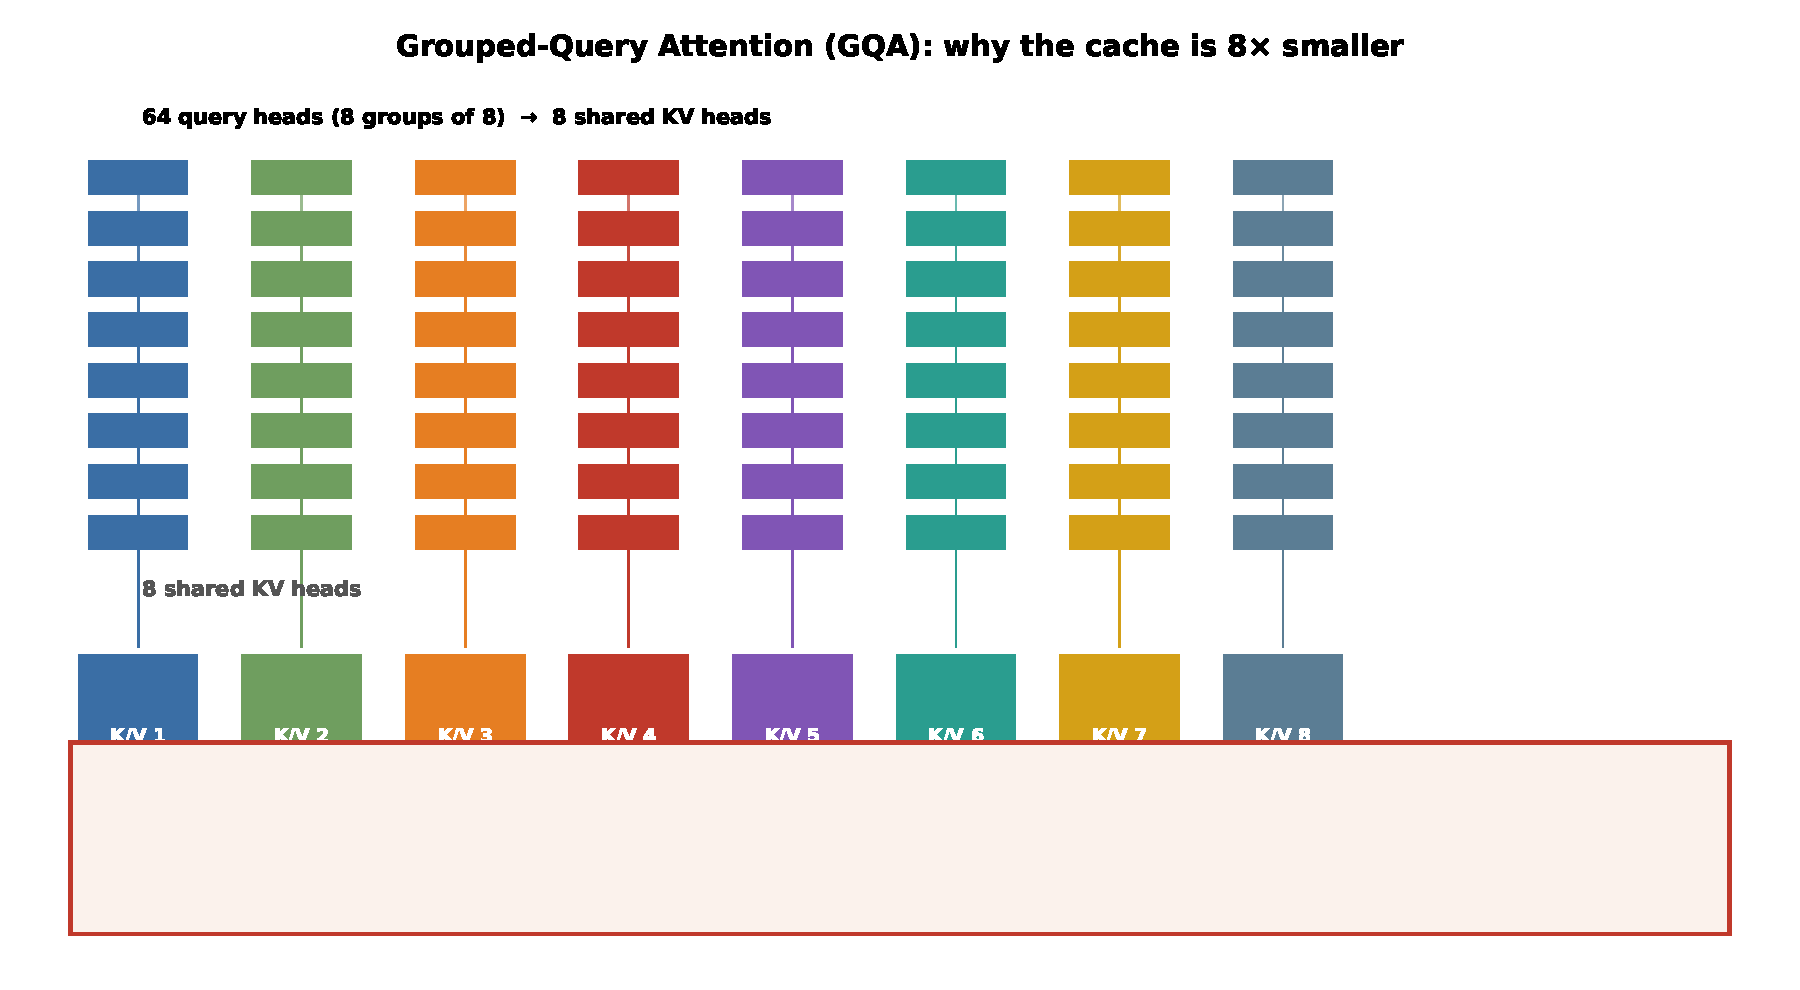
\includegraphics[keepaspectratio,alt={Fig 7.1 --- Grouped-Query Attention: 64 query heads share 8 KV heads, cutting per-token KV 8× from 2.5 MB to \textasciitilde0.33 MB (ILLUSTRATIVE, after LLaMA-2 70B head layout)},width=\maxwidth{\textwidth},keepaspectratio]{figures/fig-07-0703.pdf}}
\caption{Fig 7.1 --- Grouped-Query Attention: 64 query heads share 8 KV
heads, cutting per-token KV 8× from 2.5 MB to \textasciitilde0.33 MB
(ILLUSTRATIVE, after LLaMA-2 70B head layout)}

\label{fig:7.1}\end{figure}

\emph{\hyperref[fig:7.1]{Fig 7.1} --- The visual proof of the 8× saving. Full MHA caches a
K,V per query head (64/token → 2.5 MB/token); GQA shares one K,V across
a group of 8 query heads, so only 8 K/V per token → \textasciitilde0.33
MB/token. Head count is the real dial: substitute the model's KV-head
count into \texttt{2\ ×\ layers\ ×\ KV\_heads\ ×\ head\_dim\ ×\ bytes}.}

\textbf{\hyperref[tab:7.2]{Table 7-2}} --- Inference residency vs.~fine-tuning residency
contrast for a 70B model.

\begin{longtable}[]{@{}
  >{\raggedright\arraybackslash}p{0.2000\linewidth}
  >{\raggedright\arraybackslash}p{0.2000\linewidth}
  >{\raggedright\arraybackslash}p{0.2000\linewidth}
  >{\raggedright\arraybackslash}p{0.2000\linewidth}
  >{\raggedright\arraybackslash}p{0.2000\linewidth}@{}}
\toprule\noalign{}
\begin{minipage}[b]{\linewidth}\raggedright
scenario
\end{minipage} & \begin{minipage}[b]{\linewidth}\raggedright
memory resident
\end{minipage} & \begin{minipage}[b]{\linewidth}\raggedright
bytes per param
\end{minipage} & \begin{minipage}[b]{\linewidth}\raggedright
total (70B)
\end{minipage} & \begin{minipage}[b]{\linewidth}\raggedright
fits 8×H100 (640 GB)
\end{minipage} \\
\midrule\noalign{}
\endhead
\bottomrule\noalign{}
\endlastfoot
inference (weights + KV, 9.2K input) & weights + KV cache & FP16: 2 B;
KV adds \textasciitilde2.5 MB/token & \textasciitilde165 GB (9.2K) &
yes \\
fine-tuning (weights + gradients + optimizer) & weights + gradients +
optimizer states & Adam: \textasciitilde16 B/param (m + v + ΔW) &
\textasciitilde1,260 GB & no \\
fine-tuning (weights + gradients, FP16) & weights + gradients FP16 & 4
B/param (weights FP16 2 B + gradients FP16 2 B) & \textasciitilde280 GB
& yes \\
fine-tuning (QLoRA, 4-bit base + LoRA) & quantized base + LoRA adapters
& NF4: 4 B base; LoRA \textasciitilde5 M params & \textasciitilde50--70
GB & yes \\
inference with FP8 KV & weights FP16 + KV FP8 & KV: \textasciitilde54\%
of BF16 & \textasciitilde12.9 GB KV @ 9.2K & yes, comfortably \\

\label{tab:7.2}\end{longtable}

\emph{Inference residency = weights + KV cache; the KV footprint scales
with context length. Fine-tuning residency adds optimizer states (Adam
m, v, and updates), which for 70B at \textasciitilde16 bytes/param
exceeds 1 TB --- roughly 2× the 640 GB of 8×H100. This contrast is the
architect's central takeaway: inference is memory-limited by weights +
KV, while fine-tuning is memory-limited by weights + gradients +
optimizer, a substantially higher floor.}

\section{Measurement}\label{measurement}

Four practical measurement habits follow from the arithmetic above:

\begin{enumerate}
\def\labelenumi{\arabic{enumi}.}
\tightlist
\item
  \textbf{Compute KV-cache per-token cost for the model.} The per-token
  KV footprint of a fully-cached (MHA) attention head is
\end{enumerate}

\[
KV_{\text{per-token}} = 2 \times n_\text{layers} \times d_\text{hidden} \times \text{bytes-per-value}
\]

(one key and one value per layer, each \(d_\text{hidden}\) wide),
evaluated at the chosen precision. For a 70B model at FP16 the answer is
\(2 \times 80 \times 8192 \times 2 \text{ B} \approx 2.5\) MB/token; at
8-bit, \textasciitilde1.3 MB/token (the Ch.1 reference). Do not assume
the 1.3 MB/token figure applies at FP16 --- it does not; it is an 8-bit
number. When evaluating a model where the hidden dimension or layer
count differs from LLaMA-70B, recompute the constant factor --- a model
with 64 layers and 8192 dim will have \textasciitilde2 MB/token at FP16,
while a model with 100 layers and 12288 dim will have \textasciitilde3.7
MB/token.

\begin{enumerate}
\def\labelenumi{\arabic{enumi}.}
\setcounter{enumi}{1}
\item
  \textbf{Log peak context length, not just average.} A workload that
  averages 9.2K input tokens but has a long tail toward 32K or 128K will
  have a very different KV-cache profile. Log the 95th-percentile
  context length and re-run the KV arithmetic; the memory floor may
  shift from fitting on 2×H100 to needing 8×H100. This is especially
  important for RAG workloads, where the retrieved context may average
  8K but occasionally peak at 32K+ for technical documents.
\item
  \textbf{Measure inference residency as weights + KV, not weights
  alone.} It is common to quote only the weight footprint (140 GB for
  70B FP16) and conclude that a single H100 can hold the model. But at
  9.2K input, the KV cache adds \textasciitilde25 GB, pushing the total
  to \textasciitilde165 GB --- requiring ≥2 GPUs. Always include KV when
  we state the memory floor for inference. This measurement habit is the
  token-layer answer to the book's recurring question, ``what would I
  actually measure here?'' --- we measure token counts and their
  distribution, at the edge, before any architecture decision is made.
\item
  \textbf{Account for KV quantization when reporting residency.} If the
  serving stack uses FP8 KV (≈54\% of BF16), the per-token KV cost drops
  from \textasciitilde2.5 MB to \textasciitilde1.4 MB, and the 9.2K
  residency falls from \textasciitilde165 GB to \textasciitilde153 GB
  (weights 140 GB + KV 12.9 GB). State both the BF16 and FP8 residency
  numbers, because the choice of KV dtype changes the hardware
  requirement decisively. For comparison, 8-bit KV would bring the 9.2K
  total to \textasciitilde138 GB (weights 140 GB truncated by KV
  reduction), still fitting in 2×H100 but with less margin.
\end{enumerate}

\section{Common Mistakes}\label{common-mistakes}

\begin{itemize}
\item
  \textbf{Assuming KV-cache size scales sub-linearly.} The KV cache
  grows linearly with context length. Doubling the context from 9.2K to
  18.4K doubles the KV memory, all else equal. There is no automatic
  compression unless the attention mechanism itself is hybrid or sparse.
\item
  \textbf{Using the 8-bit KV figure (\textasciitilde1.3 MB/token) at
  FP16.} \hyperref[chap:1]{Chapter 1}'s \textasciitilde1.3 MB/token is explicitly at 8-bit
  precision. At FP16, the per-token KV cost is \textasciitilde2× that,
  ≈2.5 MB/token. Mixing the two figures produces wrong residency calls.
\item
  \textbf{Ignoring the weight + KV residency contrast.} Quoting only the
  weight footprint (140 GB for 70B FP16) and claiming it fits on one
  H100 (80 GB) is a category error. Weights alone exceed one H100; KV
  must be added.
\item
  \textbf{Treating quantization as a uniform 2×--4× reducer.} KV-cache
  quantization (FP8 ≈54\% of BF16) gives a \textasciitilde46\%
  reduction, not 2× or 4×. Weight quantization gives the larger
  reductions; do not apply the same expectation to the KV cache.
\item
  \textbf{Overlooking the fine-tuning residency floor.} Full fine-tuning
  of 70B requires \textasciitilde1.26 TB with Adam optimizer states ---
  roughly 2× 8×H100. This is not a temporary overhead; it is the
  permanent memory floor for the training duration.
\end{itemize}

\section{Architecture Consequence}\label{architecture-consequence}

The memory floor is the first constraint every architecture decision
respects, because unlike compute or bandwidth it cannot be moved by
better kernels --- it is fixed by weights + KV + (for training)
optimizer state. Several concrete consequences follow for the canonical
enterprise-Q\&A workload:

\begin{itemize}
\item
  \textbf{Model residency decides host count.} A 70B FP16 model (140 GB
  weights) at 9.2K context needs \textasciitilde24.7 GB of KV cache
  (FP16), so inference residency ≈ 165 GB --- it does \emph{not} fit on
  a single 80 GB H100, and is marginal even on 2×H100 (160 GB
  \textless{} 165 GB). The canonical single host of 8×H100 (640 GB) is
  chosen precisely to clear this floor with headroom. {[}2° DERIVED{]}
\item
  \textbf{KV-cache quantization buys back memory, not compute.} FP8 KV ≈
  54\% of BF16 (a \textasciitilde46\% reduction) {[}2°{]}, dropping 9.2K
  residency from \textasciitilde165 GB toward \textasciitilde153 GB.
  This is a \emph{memory} lever, orthogonal to bandwidth/compute fixes
  --- the architect pulls it when the KV floor, not decode bandwidth,
  binds.
\item
  \textbf{Fine-tuning is a different memory regime than inference.} The
  same model that serves in \textasciitilde165 GB demands
  \textasciitilde1,260 GB under full Adam fine-tuning (weights 140 GB +
  gradients 140 GB + optimizer states \textasciitilde1,120 GB) ---
  roughly 2× the 8×H100 host. This is why the architect separates the
  serving fleet from the training fleet: the memory floors differ by an
  order of magnitude. {[}2° DERIVED{]}
\item
  \textbf{Context length is the largest controllable KV lever.} Doubling
  context from 9.2K to 18.4K doubles KV (\textasciitilde24.7 GB →
  \textasciitilde49 GB); 128K context drives KV to \textasciitilde320
  GB, which forces quantization or model parallelism. The architecture
  must set a context-length ceiling to keep the served model within host
  memory. {[}2° DERIVED{]}
\end{itemize}

In short: the architect sizes the host by weights + KV at the longest
supported context, treats KV quantization as a spare memory dial, and
keeps inference and training on separate memory-planning tracks.

\section{What We Still Don't Know}\label{what-we-still-dont-know}

\begin{itemize}
\item
  Exact per-token KV-cache size for non-LLaMA architectures (e.g.,
  models with head\_dim ≠ 128 or 256, or attention implementations that
  store additional per-head state). The
  \texttt{2\ ×\ layers\ ×\ hidden\_dim\ ×\ bytes} formula assumes the
  standard LLaMA/llama-style key/value layout; architectures with
  grouped-query attention (GQA) or multi-query attention (MQA) may have
  fewer key/value entries per layer, changing the constant factor.
\item
  Quality loss from aggressive KV quantization (2-bit KIVI, or sub-4-bit
  schemes) at very long context lengths (128K+, MoE experts). The
  primary sources anchor FP8 KV ≈54\% of BF16 at near-zero quality loss,
  but 2-bit asymmetric patterns and their interaction with RoPE and
  sliding-window layers are not fully mapped.
\item
  Whether per-request KV caching can be partially offloaded to CPU DRAM
  during decode without TTFT impact, beyond the vLLM KV Offloading
  Connector's 2--22× TTFT reduction range which is highly
  prompt-size-dependent. The community is converging on tiered KV
  storage (GPU resident hot set + CPU/DRAM cold set), but the latency
  trade-offs at concurrency \textgreater{} 1 are not yet
  primary-anchored.
\item
  \textbf{Frontier 2026 has begun re-engineering the KV constant factor,
  not just quantizing it.} All four 2026-class open architectures attack
  KV-cache size at the attention layer itself, on top of the per-token
  footprint this chapter derives: DeepSeek-V4's hybrid CSA+HCA reports
  KV cache at only \textasciitilde10\% (Pro) / \textasciitilde7\%
  (Flash) of DeepSeek-V3.2 at 1M-token context {[}1P: arXiv
  2606.19348{]}; GLM-5.3-Flash's sparse+linear hybrid reports
  \textasciitilde4.4× KV reduction {[}1P: HF zai-org/GLM-5.3-Flash{]};
  Kimi K3's Kimi Delta Attention + Attention Residuals targets
  information flow across long sequences {[}1P: arXiv 2607.24653{]};
  Qwen3.8-Flash-Next combines Gated DeltaNet (compress history) with
  Qwen Sparse Attention (micro-block indexing) for long-context cost
  {[}1P: HF Qwen/Qwen3.8-Flash-Next{]}. For the architect this is a
  decisive shift: the KV arithmetic in this chapter (per-token ×
  context) is \emph{not} a fixed constant across model generations --- a
  2026 hybrid-attention model can hold dramatically more context per
  byte of KV than the canonical 70B/8×H100 framing assumed. Size the
  host against the \emph{specific} model's KV scheme, not a universal
  constant.
\item
  The impact of MoE routing on KV cache: does each token really emit a
  full key/value per layer across all experts, or does routing activate
  only a subset? The MoE-vs-dense facts (E1, E5) confirm that attention
  layers process every token densely and emit key/value per token, so
  MoE sparsity does not reduce KV --- but the constant factor for MoE
  models (e.g., number of experts per layer) needs per-model validation.
\end{itemize}

\subsubsection{Figures}\label{figures}

\begin{figure}
\centering
\pandocbounded{\includegraphics[keepaspectratio,alt={\hyperref[fig:7.2]{Fig 7.2} --- KV-cache size vs context length for a 70B model {[}2° DERIVED{]}},width=\maxwidth{\textwidth},keepaspectratio]{figures/fig-07-0701.pdf}}
\caption{\hyperref[fig:7.2]{Fig 7.2} --- KV-cache size vs context length for a 70B model
{[}2° DERIVED{]}}

\label{fig:7.2}\end{figure}

\emph{\hyperref[fig:7.2]{Fig 7.2} --- KV-cache growth with context length (FP16
\textasciitilde2.5 MB/token, FP8 \textasciitilde1.4, 8-bit
\textasciitilde1.3); at 128K the FP16 KV footprint climbs to
\textasciitilde320 GB, approaching the \textasciitilde436 GB KV budget
only well beyond 128K, and already reaches \textasciitilde165 GB
inference residency at 9.2K.}

\begin{figure}
\centering
\pandocbounded{\includegraphics[keepaspectratio,alt={\hyperref[fig:7.3]{Fig 7.3} --- Inference vs fine-tuning memory floor {[}2° DERIVED{]}},width=\maxwidth{\textwidth},keepaspectratio]{figures/fig-07-0702.pdf}}
\caption{\hyperref[fig:7.3]{Fig 7.3} --- Inference vs fine-tuning memory floor {[}2°
DERIVED{]}}

\label{fig:7.3}\end{figure}

\emph{\hyperref[fig:7.3]{Fig 7.3} --- The same 70B model serves in \textasciitilde165 GB
(weights + KV) but needs \textasciitilde1,260 GB for full Adam
fine-tuning; QLoRA fits \textasciitilde50--70 GB on a single GPU.}

\begin{figure}
\centering
\pandocbounded{\includegraphics[keepaspectratio,alt={\hyperref[fig:7.4]{Fig 7.4} --- The concurrency budget: where a 70B host's 640 GB pool goes {[}2° DERIVED{]}},width=\maxwidth{\textwidth},keepaspectratio]{figures/fig-07-0704.pdf}}
\caption{\hyperref[fig:7.4]{Fig 7.4} --- The concurrency budget: where a 70B host's 640 GB
pool goes {[}2° DERIVED{]}}

\label{fig:7.4}\end{figure}

\emph{\hyperref[fig:7.4]{Fig 7.4} --- Where a serving host's 640 GB pool goes. 140 GB
weights + \textasciitilde64 GB runtime/NCCL leaves \textasciitilde436 GB
of KV budget; at 23.8 GB/request (FP16) that is C ≈ 18 concurrent
requests, and FP8 (\textasciitilde12.4 GB/request) roughly doubles it to
\textasciitilde35. This is the arithmetic behind the single-host
capacity in Ch17.}

\begin{figure}
\centering
\pandocbounded{\includegraphics[keepaspectratio,alt={\hyperref[fig:7.5]{Fig 7.5} --- Memory Tetris: how the 8×H100 host's 640 GB pool fills at three contexts (9.2K / 32K / 128K). Runtime \textasciitilde64 GB + weights 140 GB + KV cache 23.8 / 80 / 320 GB {[}2° DERIVED{]}},width=\maxwidth{\textwidth},keepaspectratio]{figures/fig-07-0705.pdf}}
\caption{\hyperref[fig:7.5]{Fig 7.5} --- Memory Tetris: how the 8×H100 host's 640 GB pool
fills at three contexts (9.2K / 32K / 128K). Runtime \textasciitilde64
GB + weights 140 GB + KV cache 23.8 / 80 / 320 GB {[}2° DERIVED{]}}

\label{fig:7.5}\end{figure}

\emph{\hyperref[fig:7.5]{Fig 7.5} --- The Memory Tetris: why context length is the ultimate
memory lever. The 640 GB pool stacks \textasciitilde64 GB runtime/NCCL +
140 GB weights, leaving \textasciitilde436 GB of headroom. The FP16 KV
cache (orange) is the only block that grows with context --- 23.8 GB at
9.2K, 80 GB at 32K, \textasciitilde320 GB at 128K. Because the KV budget
is fixed (\textasciitilde436 GB), longer context consumes it outright:
at 9.2K it supports \textasciitilde18 concurrent, but 128K leaves room
for only \textasciitilde1--2. This is what makes the KV constant (Ch7
§3) the single most capacity-relevant number in a serving design. {[}2°
DERIVED{]}}

\section{End-of-Chapter Mini-Case}\label{end-of-chapter-mini-case}

An architect is asked to design an internal Q\&A system over the
company's document repository. The initial ask is vague: ``We need to
let all 5,000 employees ask questions over our internal wikis.'' Before
any architecture can be defended, the architect must turn this vague
desire into a machine-denominated statement using the chapter's core
constraint.

From the token layer alone (which we worked through in this chapter),
the architect can already establish several facts. The unit is tokens;
the request shape will be prompt + retrieved context + output; the
workload is input-heavy (retrieved context dominates); and the first
number to lock down is tokens-per-request, because every downstream
decision (which model fits, how much memory, what latency is possible)
is priced against it.

Running the KV arithmetic: if each request uses \textasciitilde9.2K
retrieved context tokens (the canonical \textasciitilde1,200 prompt + 8K
retrieved) plus \textasciitilde300 output tokens, the KV cache per
request at 70B FP16 is \textasciitilde24.7 GB. The weight footprint is
140 GB. Total inference residency ≈ 165 GB, which fits in 2×H100 (160
GB) with a small margin, or comfortably in 8×H100 (640 GB). If the
context is extended to 32K (e.g., wider document retrieval), the KV
cache rises to \textasciitilde80 GB, pushing total residency to
\textasciitilde220 GB --- still fitting in 8×H100 but requiring a
multi-GPU node.

The architect can now speak the system's currency: tokens, KV bytes, and
the residency floor. The next step --- turning ``5,000 employees'' into
\textasciitilde2,000 concurrent users, \textasciitilde10 requests/s, and
a specific model-and-hardware choice --- is \hyperref[chap:4]{Chapter 4}'s job (workload
anatomy). Here the point is narrower and sharper: we can now say, with
quantified memory numbers, whether the system fits on the available
hardware, and we can compare inference vs.~fine-tuning residency floors
before committing to a architecture decision. This is the chapter's
payoff: the vague request has been translated into concrete constraint
numbers, and the architect can defend a recommendation based on whether
the workload fits, not on intuition alone.
